\section{Architecture}

The final architecture of our project is similar to the one we presented in our midterm project. As the specification requires, the \texttt{gossip} module runs as two independent protocols: one API protocol and one P2P protocol. These two protocols share some data to fulfill the functionality of the module.

\begin{figure}[H]
    \centering
    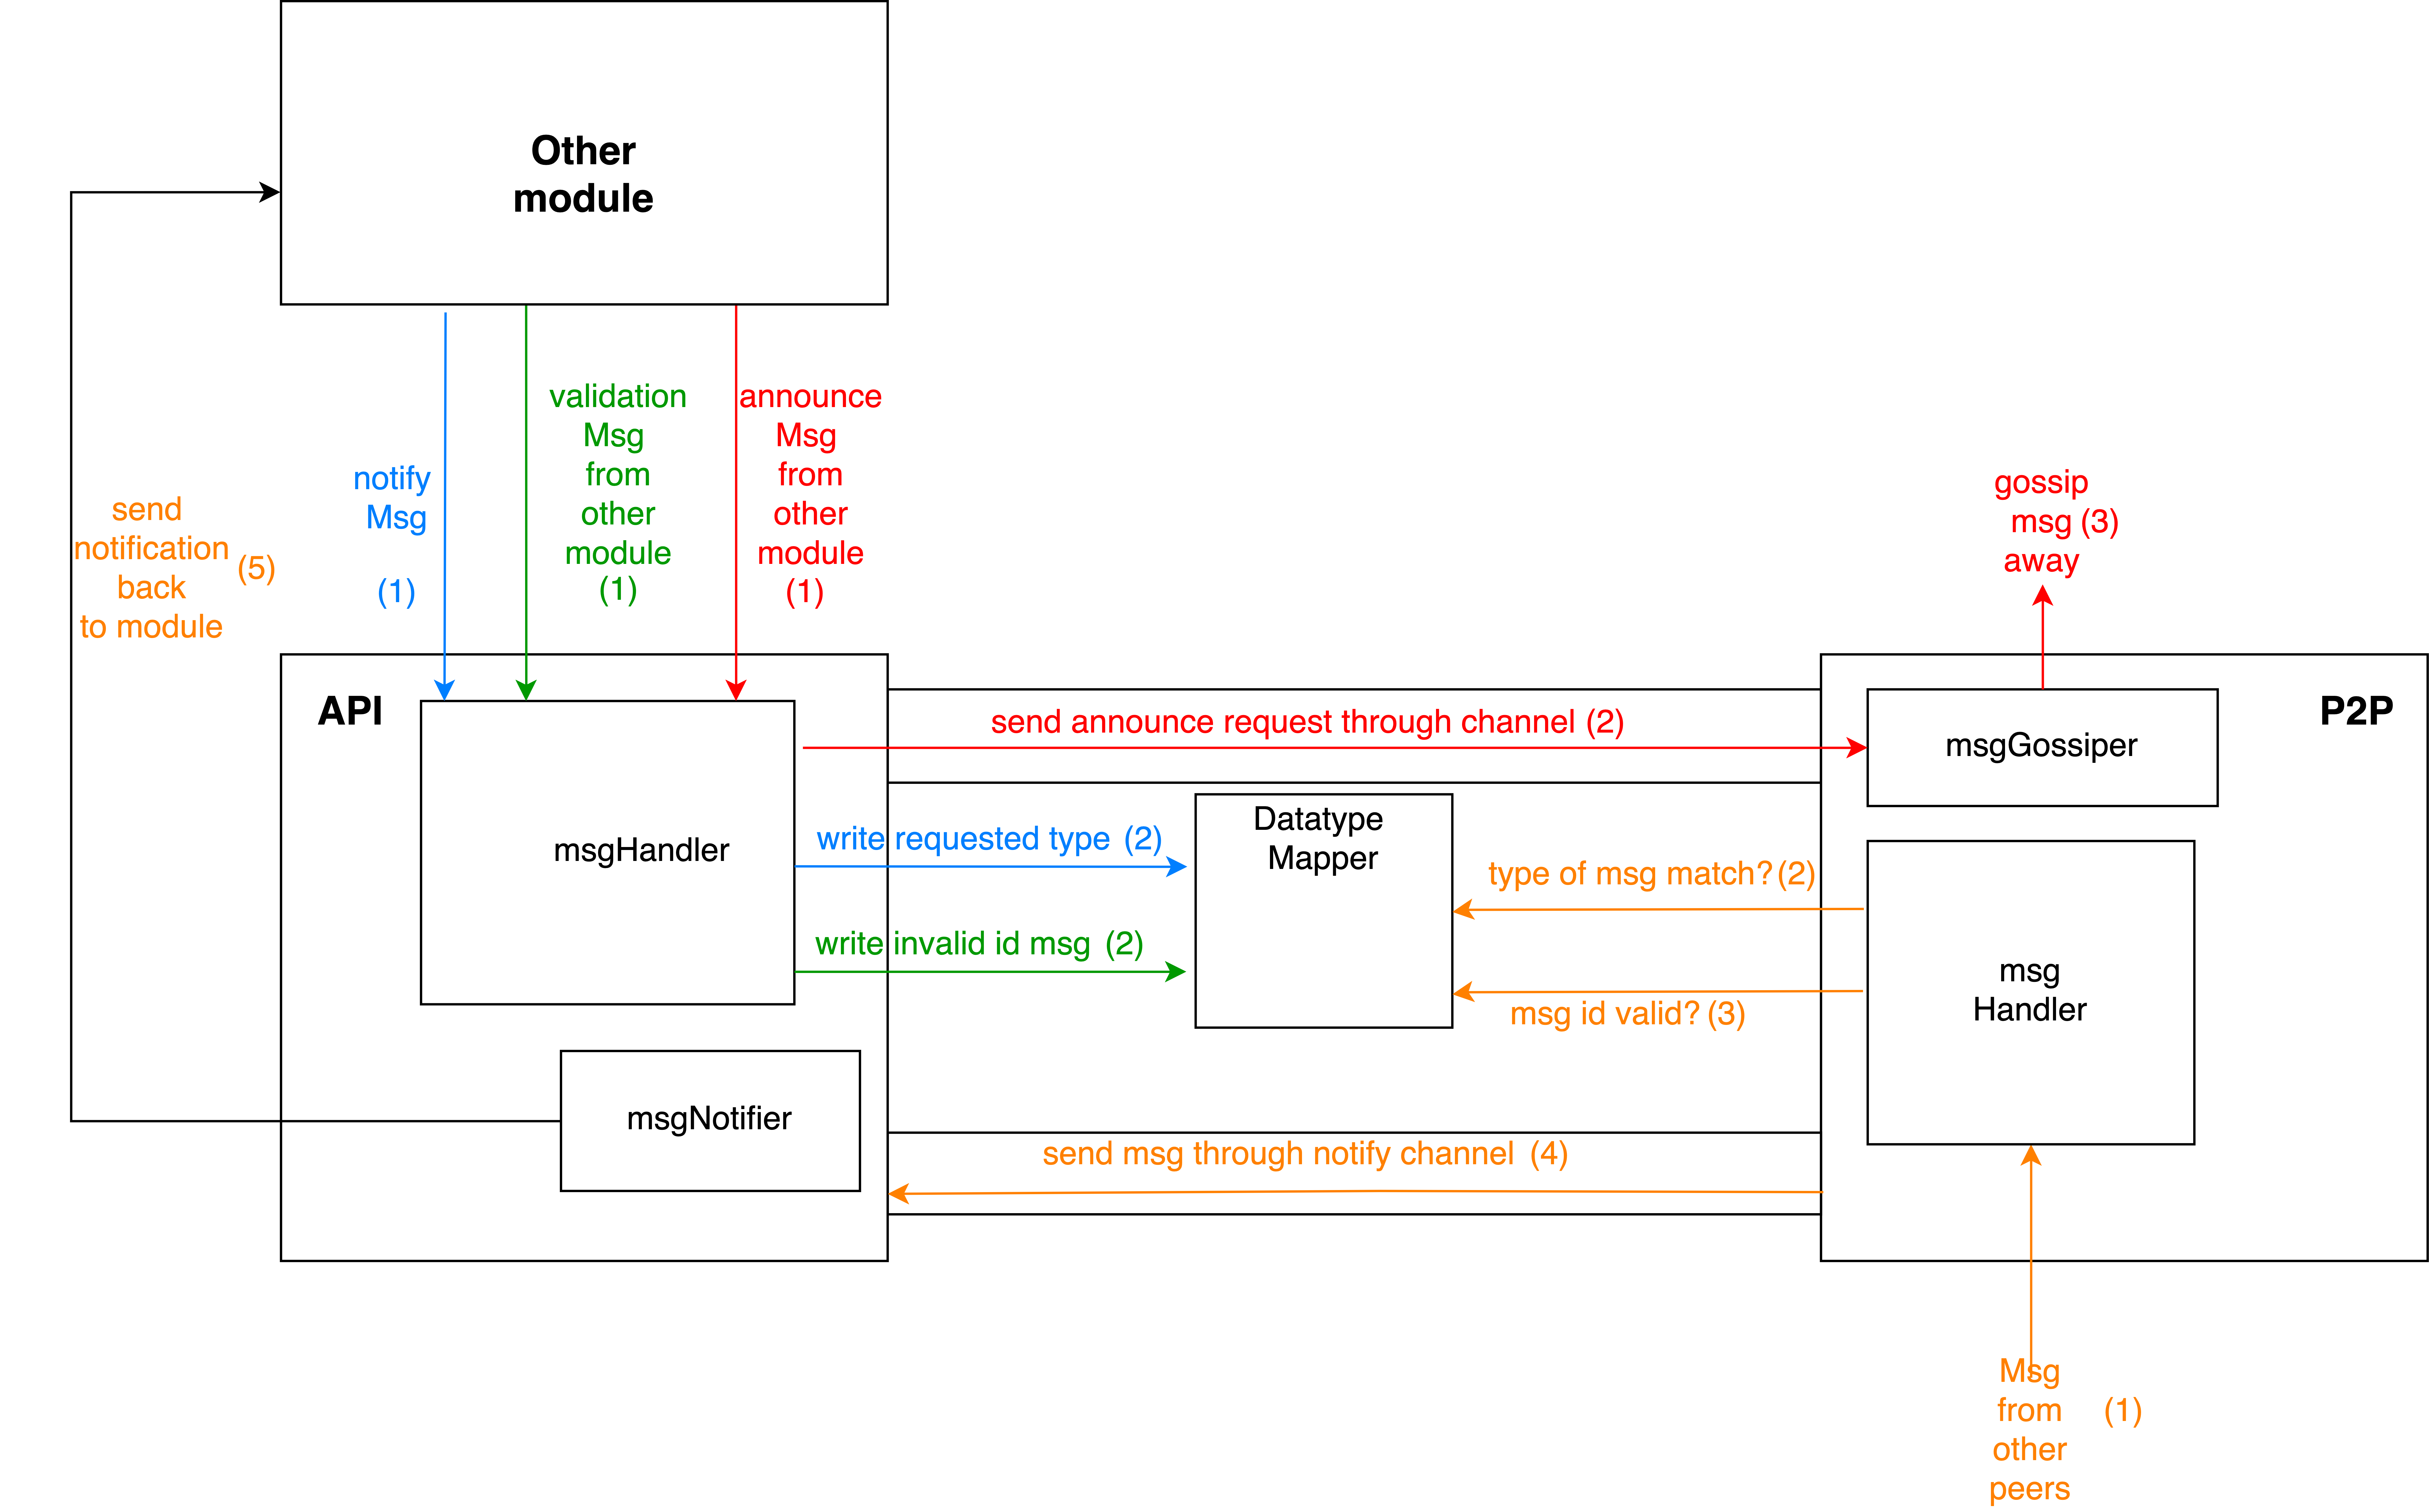
\includegraphics[width=0.85\textwidth]{pics/architecture.png}
    \caption{Structure of the gossip module}
    \label{fig:architecture}
\end{figure}

\subsection{Shared data between API and P2P}

\subsubsection{AnnounceMsgChan}

We have an announce \texttt{Go channel}~\parencite{goChannel} (marked in red in Figure \ref{fig:architecture}) shared between the two protocols. Whenever the \texttt{API} protocol receives an announce message from another module, it processes the message immediately and sends it to the \texttt{P2P} protocol through this channel. The \texttt{P2P} protocol has an announce message handler running on a goroutine that always listens to this channel. When it receives an announce request, it will gossip this message away. 

\subsubsection{DatatypeMapper}

We also need a \texttt{DatatypeMapper} (marked in black in Figure \ref{fig:architecture}) shared between two protocols. Whenever API receives a notify message, it will write the message type that is valid into the mapper and hence should be propagated further. \texttt{DatatypeMapper} also contain a list of invalid message id, which is sent by other module through \texttt{Validation} endpoint. This list is being used by \texttt{P2P} to check for the validity of a message before forwarding it through \texttt{NotiyiMsgChan} 

This datatype mapper will, of course, own a mutex that guarantees no race condition between the two protocols.

\subsubsection{NotiyiMsgChan}

Thanks to the \texttt{DatatypeMapper}, the \texttt{P2P} protocol can recognize which kind of message it should propagate. When it receives a new message, it will check if this message type was requested by any module by reading the datatype mapper and if the message is valid. If that is the case, it sends this message through \texttt{NotiyiMsgChan} (marked in orange in Figure \ref{fig:architecture}). \texttt{API} protocol also has a running goroutine that constantly listens to this channel. It can get those messages from P2P and send corresponding notification messages to the module requesting them. 

\subsection{Security}

We changed our security mechanism according to our midterm feedback. We integrated \texttt{POW} in every gossip message. The hardness of this challenge is defined in the config file. Depending on the security requirement of the project, we can adjust the hardness, also known as the number of leading zeros, accordingly. 

\section{Software Documentation}

\subsection{Dependency}

\subsection{How to install and run}

\subsection{Known Issues}

\section{Future Work}

\section{Workload distribution}

